\section{Physical Implementation}
\label{sec:PCB-implementation}

The final, delivered module is a $90mm\times62mm$ PCB. The PCB manufactured 
for the project was done so for free, using Spirit Circuits' "Go Naked"
service \cite{go-naked}. The PCB itself is a "tracks and holes" only service 
- no soldermask or silkscreen is applied. The schematic of the circuit 
delivered is available in Appendix ???, and of the PCB layout in Appendix 
???. A waterproof lacquer will be applied to the PCB to prevent condensation 
from shorting tracks together, and the module itself presented in a 
waterproof container before flight testing.

\begin{figure}[H]
        \centering
        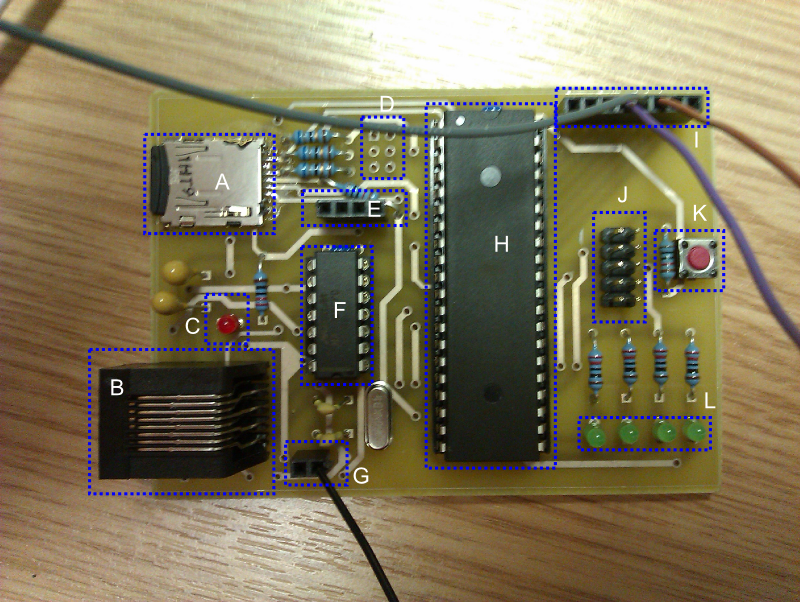
\includegraphics[width=1.00\textwidth]{figures/PayloadImplementationA.png}
        \captionof{figure}{Image of the final payload, under test, before lacquer is applied. R11 can be seen between the Camera header and a via near the SD card Vcc.}. 
        \label{fig:PayloadImplementation}
\end{figure}

In figure \ref{fig:PayloadImplementation}, the letters refer to the following 
features of the payload module:

\begin{itemize}
\item \textbf{A:} microSD Card slot
\item \textbf{B:} RJ45 socket, more popularly known as an ethernet socket. 
(Actually implements the RS485 protocol)
\item \textbf{C:} Power LED. Shows whether 3V3 from the ethernet socket is connected.
\item \textbf{D:} ISP programming header socket. As seen, this is not 
soldered on, as we have been using the JTAG header, but will be soldered 
before delivery to the customer.
\item \textbf{E:} Camera header. The camera can be connected to our PCB 
simply by attaching the hook-up wire in the correct order. (L-R: 3V3, GND, 
Camera TX, Camera RX)
\item \textbf{F:} MAX489 (RS485 Transceiver) \footnote{\url{http://uk.farnell.com/9725148}}. 
Cheaper version of the MAX3070 used in the sample peripheral.
\item \textbf{G:} Power header. L: 3V3, R: GND.
\item \textbf{H:} ATmega644P \cite{atmega644p}
\item \textbf{I:} ATmega644P Port A expansion header. (In the image, this is 
being used as a connection to an Arduino Uno so that we may view the debug 
information)
\item \textbf{J:} JTAG programming header
\item \textbf{K:} Reset button
\item \textbf{L:} Debug LEDs
\end{itemize}

Due to an issue discovered between ordering and receiving the PCB, an 
additional 10k$\Omega$ resistor has been placed between Camera RX and 3V3 (R11 
on the schematic). Also, the Single In Line header holes (for the Port A 
expansion and camera headers) have been widened from 0.40mm to 0.80mm. An 
update to the PCB layout is provided in the delivered repository.

The camera will also be presented in a sealed, weatherproof container.
